\section{Die Layout-Manager}

In diesem Kapitel werden die Layout- oder Gemeometrie-Manager von Tkinter behandelt.
Grunds�tzlich stehen drei verschiedene Layout-Manager zur Verf�gung:

\begin{description}
    \item Pack
    \item Grid
    \item Place
\end{description}

Layout-Manager dienen in erster Linie dazu, Widgets in einem Wurzel-Element zu regestrieren,
anzuordnen und darzustellen. Besonders die Anordnung durch Angabe von Position und Gr��e eines Widgets
wird durch die Layout-Manager stark vereinfacht.

Einem Wurzel-Element sollte immer nur ein Layout-Manager angeh�ngt werden.

\subsection{Pack}

Der Pack-Manager ist der am einfachsten zu verwendende Layout-Manager.
Hier werden Widgets in Zeilen oder Spalten 'gepackt' und durch Optionen wie
\lstinline$fill$ oder \lstinline$expand$ gesteuert.

Im Vergleich zu dem sehr �hnlichen Grid-Manager ist der Pack-Manager etwas eingeschr�nkt,
aber in einigen wenigen Situationen sinnvoller zu nutzen. Speziell wenn einfache
Widgets �bereinander oder nebeneinander angeordnet werden, oder Inhalte eines Widgets das gesamte
�bergeordnete Widget ausf�llen sollen wird der Pack-Manager bevorzugt.

Das folgende Beispiel soll die Effekte des Pack-Managers verdeutlichen:

\lstinputlisting[language=Python]{chapters/userInterface/src/GUI_PackExample.py}
\label{gui:gui_packexample}

\begin{figure}[ht]
	\centering
	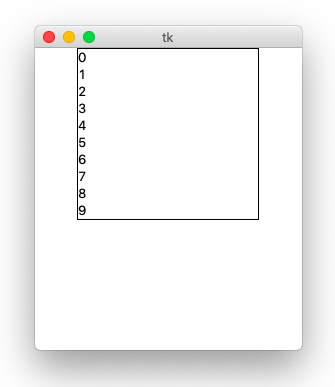
\includegraphics[width=0.8\textwidth]{images/PackManagerGUI_II.png}
	\caption{Listbox Widget mit einem Pack-Manager angeordnet}
	\label{fig:PackManagerGUI_I}
\end{figure}

\newpage

Standardm��ig wird die Gr��e der Listbox so gew�hlt, dass Zehn Elemente angezeigt
werden k�nnen. Im obigen Quelltext werden der Listbox allerdings doppelt so viele Elemente
�bergeben. Versucht der User nun das Wurzel-Element, sprich das Fenster, zu verg��ern
um alle Elemente anzuzeigen, erzeugt Tkinter rund um das Listbox-Widget einen Abstand zum Fenster.
Um das Widget der gesamten zur Verf�gung stehenden Fl�che anzupassen, m�ssen die
Optionen \lstinline$fill$ und \lstinline$expand$ des Pack-Managers angesprochen werden.

\lstinputlisting[language=Python]{chapters/userInterface/src/GUI_PackExampleII.py}
\label{gui:gui_packexample}

\begin{figure}[ht]
	\centering
	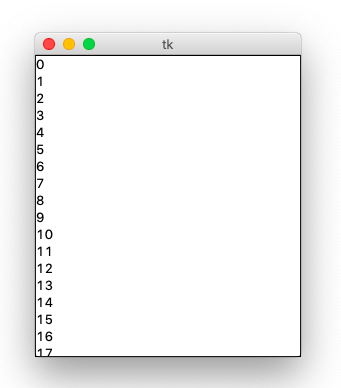
\includegraphics[width=0.8\textwidth]{images/PackManagerGUI_I.png}
	\caption{Listbox Widget mit einem Pack-Manager angeordnet unter Angabe von fill und expand}
	\label{fig:PackManagerGUI_II}
\end{figure}

Die \lstinline$fill$-Option teilt dem Pack-Manager mit, dass der gesamte zur Verf�gung
stehende Raum durch das Widget ausgef�llt werden soll. Der dahinter stehende Wert
regelt wie der Raum gef�llt wird. \lstinline$BOTH$ bedeutet, dass das Widget
sowohl horizontal als auch vertikal expandierten soll.
Alternativ kann der Raum mit der Angabe \lstinline$X$ nur horizontal und mit der Angabe
\lstinline$Y$ nur vertikal ausgef�llt werden.
